\chapter{视频录屏}
\begin{align*}
    A + B = C
\end{align*}

\begin{equation*}
    A + B = C
\end{equation*}

\begin{align*}
    A + B & = C \\
    C - A & = B
\end{align*}

\begin{equation*}
    A + B = C \\
    C - A = B
\end{equation*}

\begin{align}
    A + B & = C \\
    C - A & = B
\end{align}

\begin{equation}
    \begin{aligned}
    A + B & = C \\
    A + B & = C \\
    A + B & = C \\
    A + B & = C \\
    C - A & = B
    \end{aligned}
\end{equation}

\begin{subequations}
\begin{equation}
    A + B = C
\end{equation}
\begin{equation*}
    A + B = C
\end{equation*}
\begin{equation}
    A + B = C
\end{equation}
\end{subequations}

\begin{center}
\begin{tabular}{|c|c|c|c|c|}
\hline
    $A_1$ & A2 & A3 & A4 &A5 \\
    \hline
    $B_1$ & B2 &B3 & B4 &B5 \\
    \hline
    $C_1$ & C2 & C3 & C4 &C5 \\
    \hline
\end{tabular}    
\end{center}


\begin{center}
\begin{tabular}{|m{2cm}<\centering|m{2cm}<\centering|m{2cm}<\centering|m{2cm}<\centering|m{2cm}<\centering|}
\hline
    $A_1$ & A2 & A3 & A4 &A5 \\
    \hline
    $B_1$ & B2 &B3 & B4 &B5 \\
    \hline
    $C_1$ & C2 & C3 & C4 &C5 \\
    \hline
\end{tabular}    
\end{center}


\begin{center}
\captionof{table}{例表}
\begin{tabular}{|m{2cm}<\centering|m{2cm}<\centering|m{2cm}<\centering|m{2cm}<\centering|m{2cm}<\centering|}
\hline
    {\cellcolor{blue!25}$A_1$} & A2 & A3 & A4 &A5 \\
    \hline
    $B_1$ & B2 &B3 & B4 &B5 \\
    \hline
    $C_1$ & C2 & C3 & C4 &C5 \\
    \hline
\end{tabular}    
\end{center}

\begin{table}[t]
    \centering
    \caption{例表}
\begin{tabular}{|m{2cm}<\centering|m{2cm}<\centering|m{2cm}<\centering|m{2cm}<\centering|m{2cm}<\centering|}
\hline
    {\cellcolor{blue!25}$A_1$} & A2 & A3 & A4 &A5 \\
    \hline
    $B_1$ & B2 &B3 & B4 &B5 \\
    \hline
    $C_1$ & C2 & C3 & C4 &C5 \\
    \hline
\end{tabular} 
\end{table}

\begin{center}
\textit{}    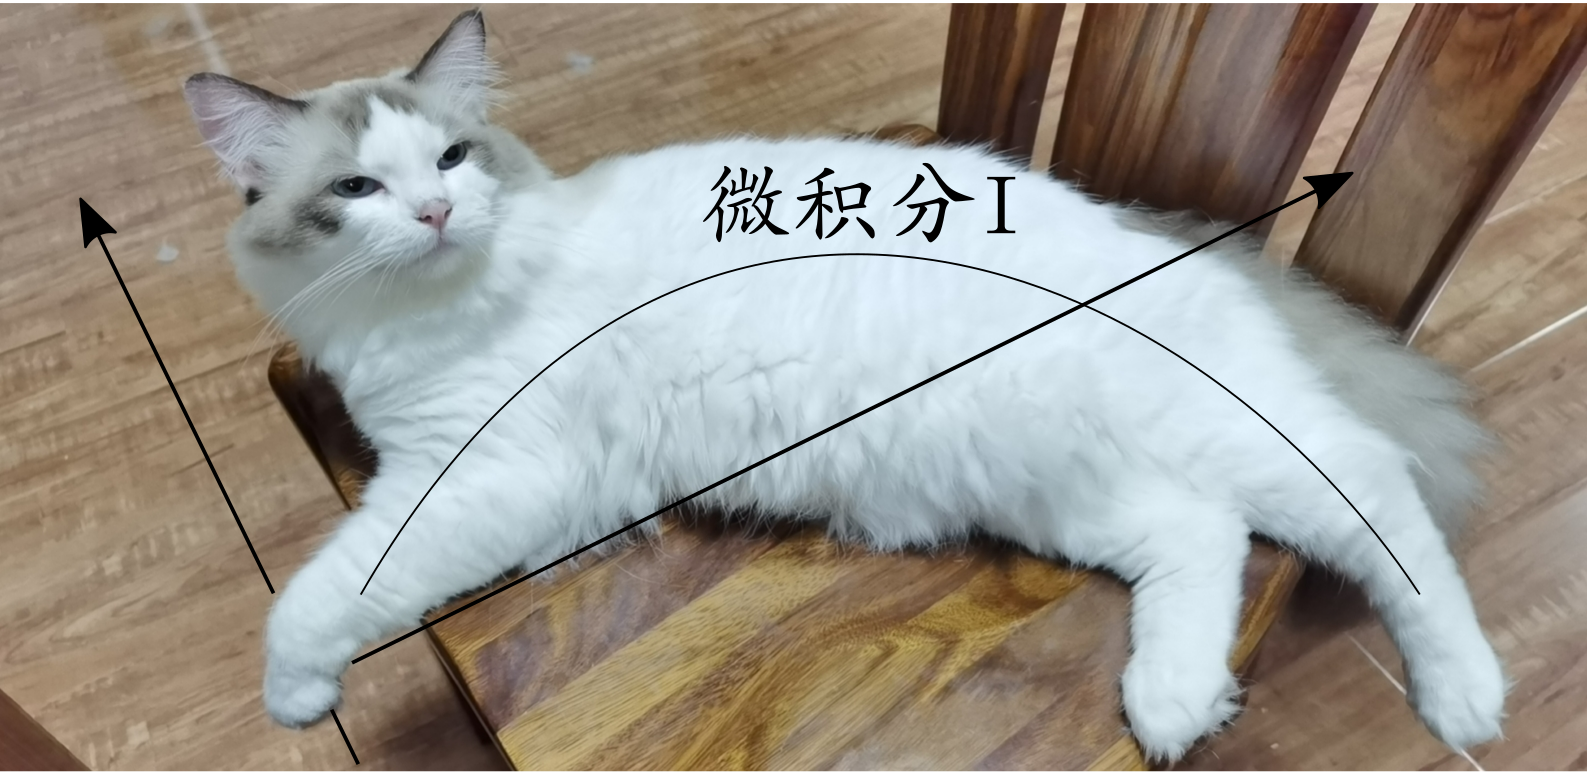
\includegraphics[scale=0.6]{figure/Ragdoll.png}
    \captionof{figure}{Ayumu的猫}
\end{center}

\begin{figure}[b]
    \centering
    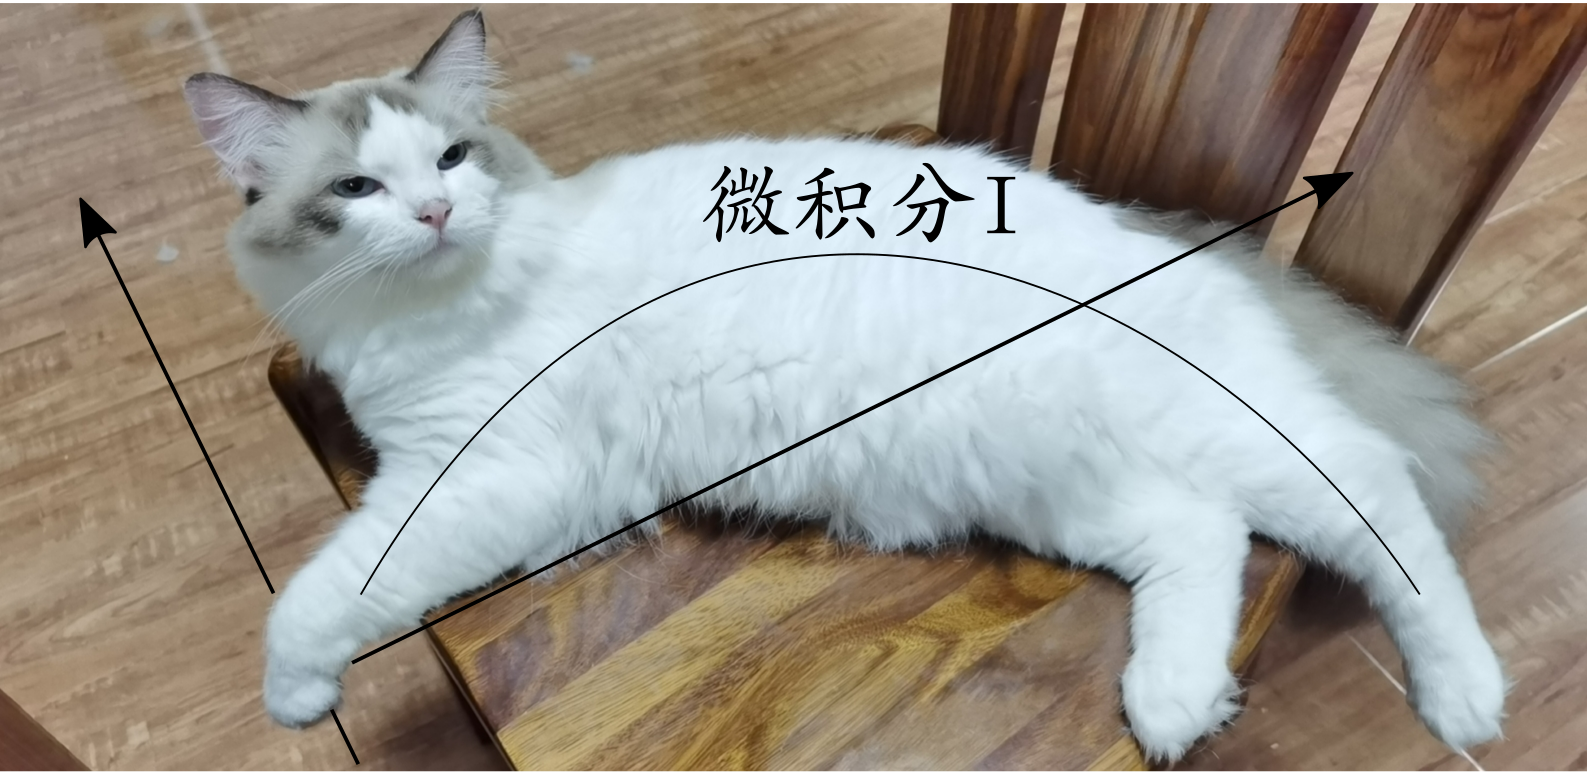
\includegraphics[scale=0.6]{figure/Ragdoll.png}
    \caption{Ayumu的猫}
\end{figure}

\begin{center}
    \includesvg[scale =0.25]{figure/Ragdoll.svg}
    \captionof{figure}{Ayumu的猫}
\end{center}


\begin{center}
    \def\svgwidth{0.7\columnwidth}
    \input{figure/Ragdoll.pdf_tex}
    \captionof{figure}{Ayumu的猫}
\end{center}

\begin{theorem}
\begin{center}
    \def\svgwidth{0.7\columnwidth}
    \input{figure/Ragdoll.pdf_tex}
    \captionof{figure}{Ayumu的猫}
\end{center}
\end{theorem}

\begin{theorem}
\begin{minipage}{0.5\textwidth}
猫猫猫猫 布偶猫
\end{minipage}
\begin{minipage}{0.5\textwidth}
\begin{center}
    \def\svgwidth{0.7\columnwidth}
    \input{figure/Ragdoll.pdf_tex}
    \captionof{figure}{Ayumu的猫}
\end{center}
\end{minipage}
\end{theorem}